\newpage
\section{Simulation}

\subsection{Erläuterung zu der Simulation}
Die Antenne wurde über mehrere Simulationsschritte verfeinert, so dass sie das gewünschte Verhalten aufzeigt.\\ 
Gemäss Simulation sollte die Antenne einen Reflexionsfaktor von knapp -25dB aufweisen bei einer Frequenz von 2.4GHz. Bei 5 GHz sollte dieser bei -17dB liegen. Abbildung \ref{fig:reflexionsfaktor} auf Seite \pageref{fig:reflexionsfaktor}.\\
Die reale Impedanz liegt gemäss Simulation bei 2.4 GHz bei 43 Ohm, der Imaginäranteil bei 10 Ohm kapazitiv. Bei 5 GHz liegt der Realanteil bei 40 Ohm und der Imaginäranteil bei 6 Ohm. Abbildung \ref{fig:impedanz} auf Seite \pageref{fig:impedanz}.\\
Auf Seite \pageref{fig:electricfield} sind in Abbildungen \ref{fig:electricfield_2_4} und \ref{fig:electricfield_5_0} das elektrische Feld für 2.4GHz und 5 GHz abgebildet. Die Simulation zeigt schön, wie sich das elektrische Feld je nach Frequenz unterschiedlich ausprägt.\\
Auch die Simulation für die Oberflächenstromdichte zeigt ein ausgeprägtes Verhalten, je nach angelegter Frequenz. Abgebildet auf Seite \pageref{fig:currentdensity} in Abbildungen \ref{fig:currentdensity_2_4} und \ref{fig:currentdensity_5_0}.


\clearpage
\subsubsection{Reflexionsfaktor $S_{11}$}
\begin{figure}[h!]
	\centering
	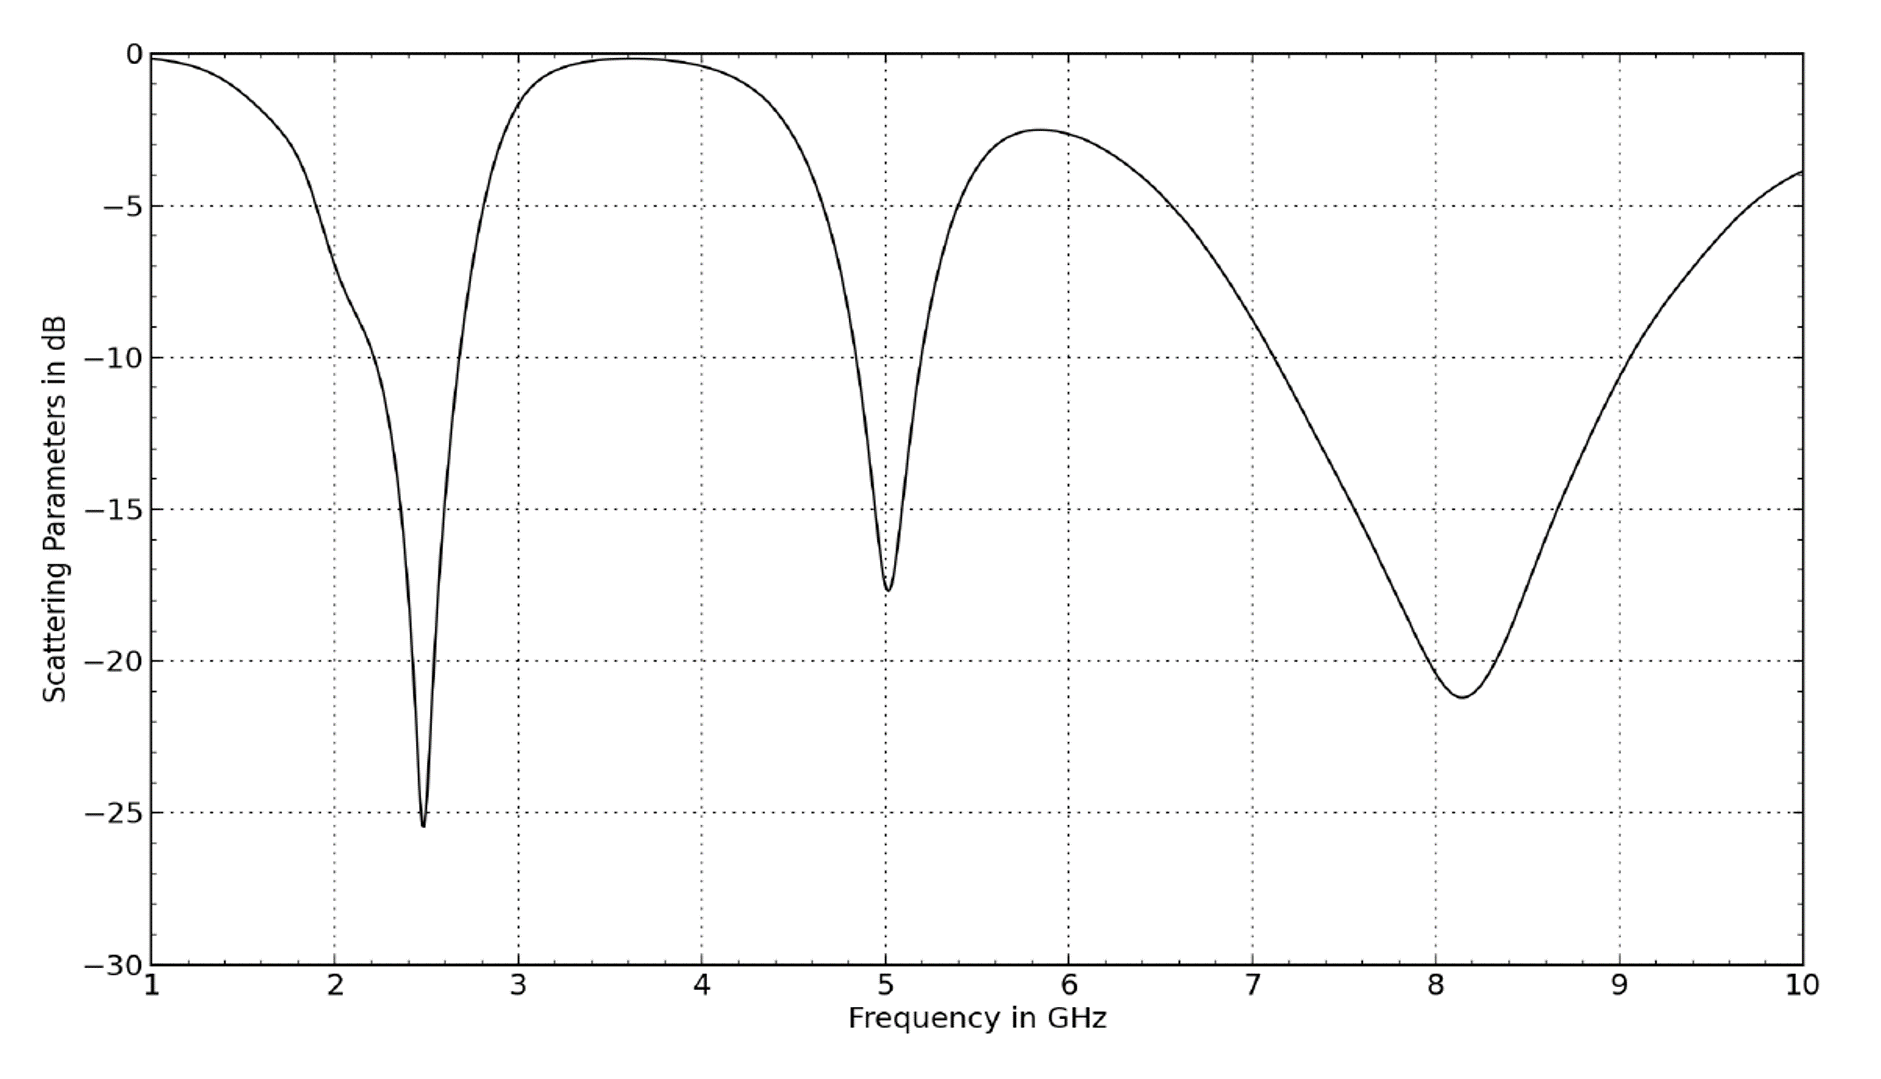
\includegraphics[width=0.7\textwidth]{../fig/plt/crazy_stuff_l4_pcb_v2c_laptop_1a_105_S11_2.png}
	\caption{Reflexionsfaktor $S_{11}$}
	\label{fig:reflexionsfaktor}
\end{figure}

%\clearpage
\subsubsection{Impedanz}
\begin{figure}[h!]
	\centering
	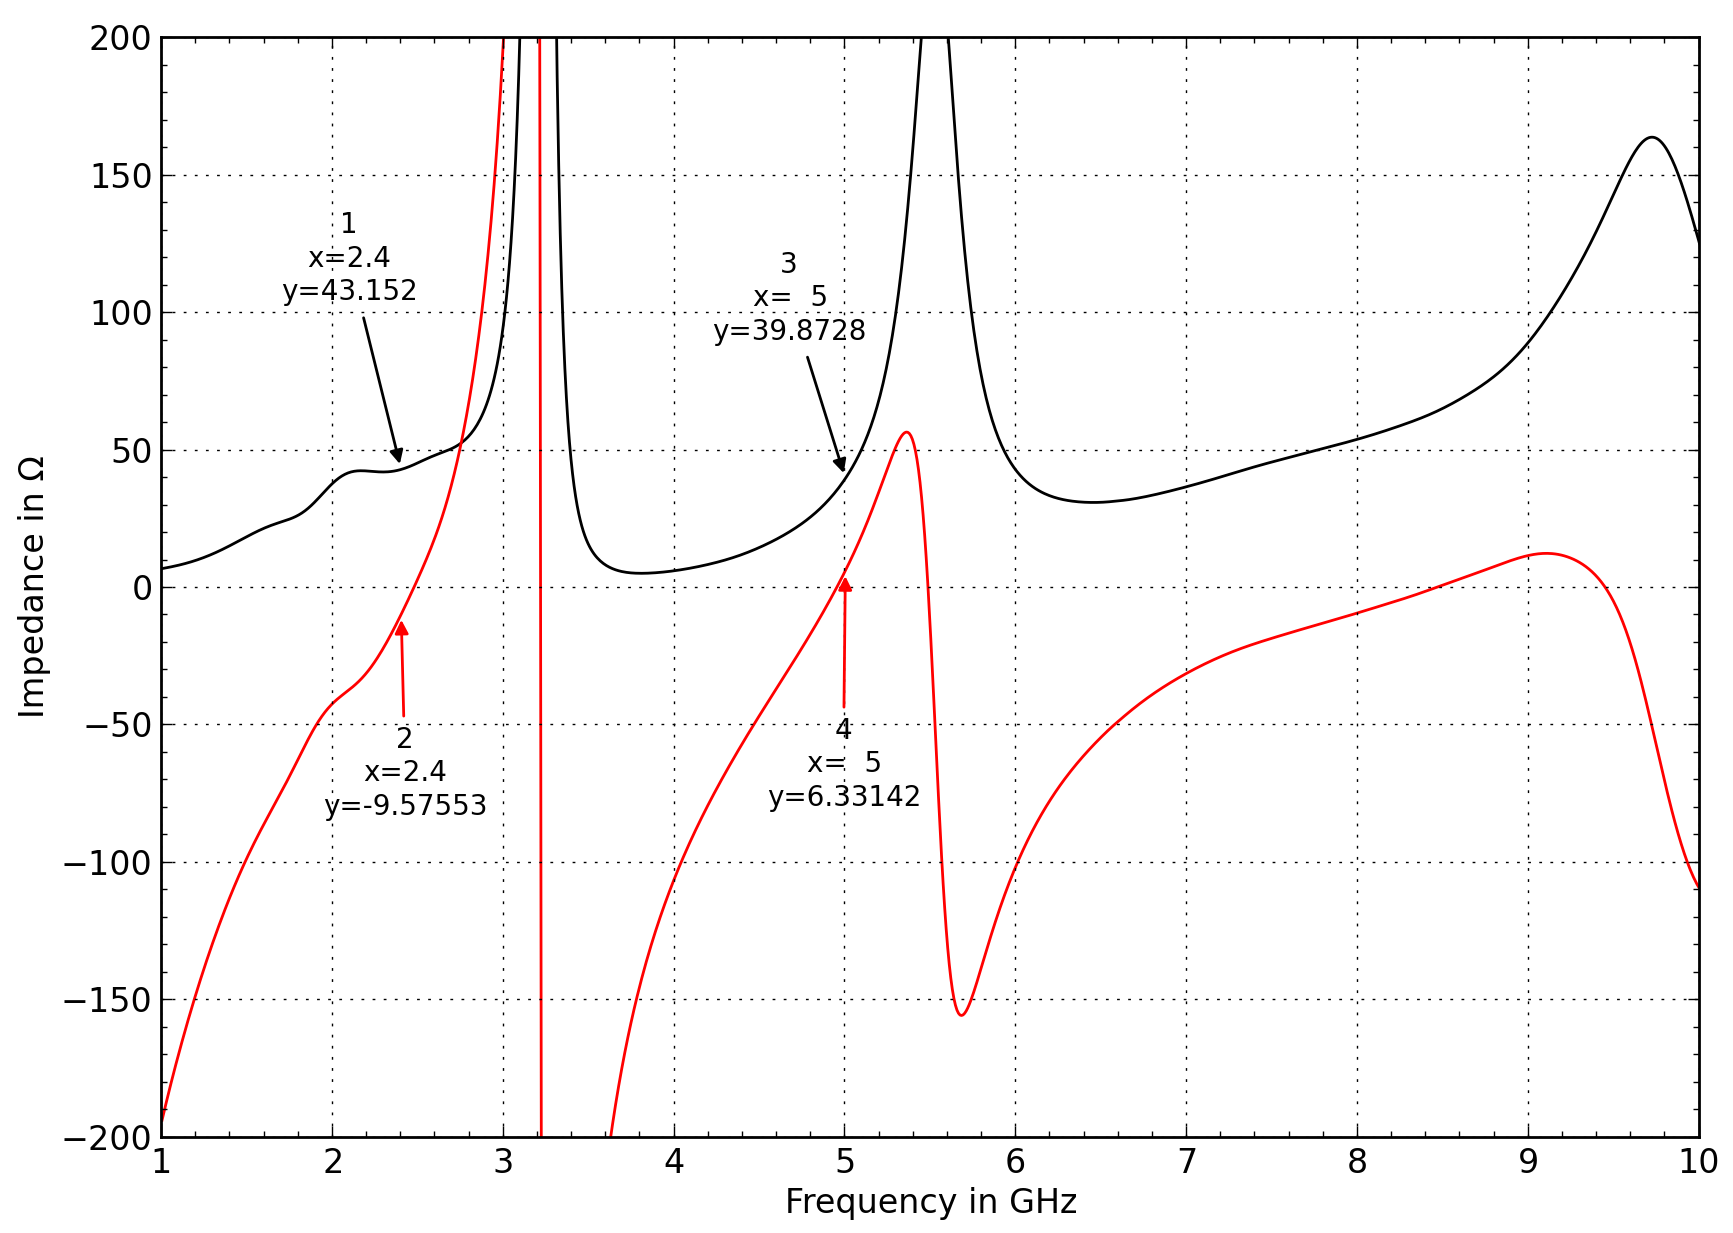
\includegraphics[width=0.7\textwidth]{../fig/plt/crazy_stuff_l4_pcb_v2c_laptop_1a_105_Widerstand_1.png}
	\caption{Impedanz}
	\label{fig:impedanz}
\end{figure}

\newpage
\subsubsection{Elektrisches Feld}
\begin{figure}[h!]
	\begin{center}
		\begin{subfigure}[t]{0.49\textwidth}
			\begin{center}
				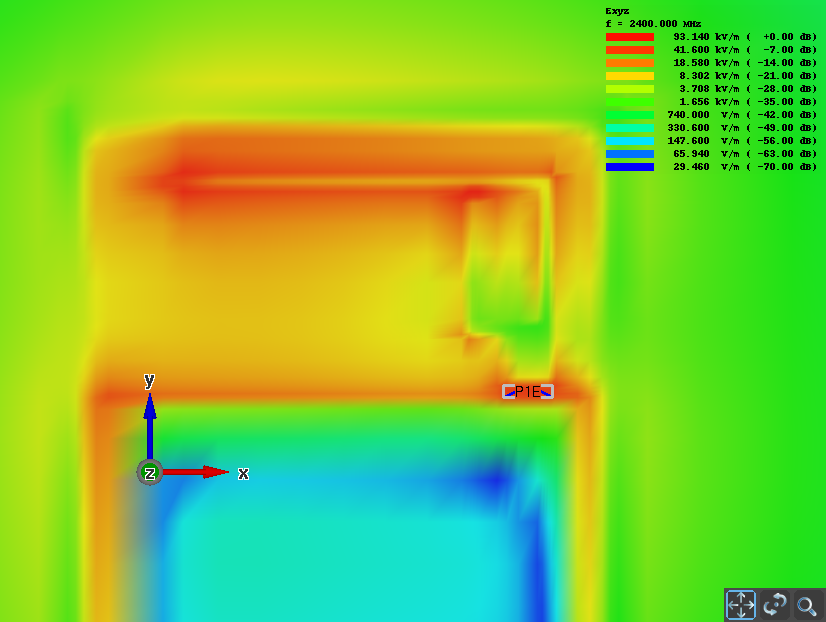
\includegraphics[width=0.94\textwidth]{../fig/plt/crazy_stuff_l4_pcb_v2c_laptop_1a_105_2ghz4_3d_electric_field_xy.png}
				\caption{bei 2.4 GHz}
				\label{fig:electricfield_2_4}
			\end{center}
		\end{subfigure}
		\begin{subfigure}[t]{0.49\textwidth}
			\begin{center}
				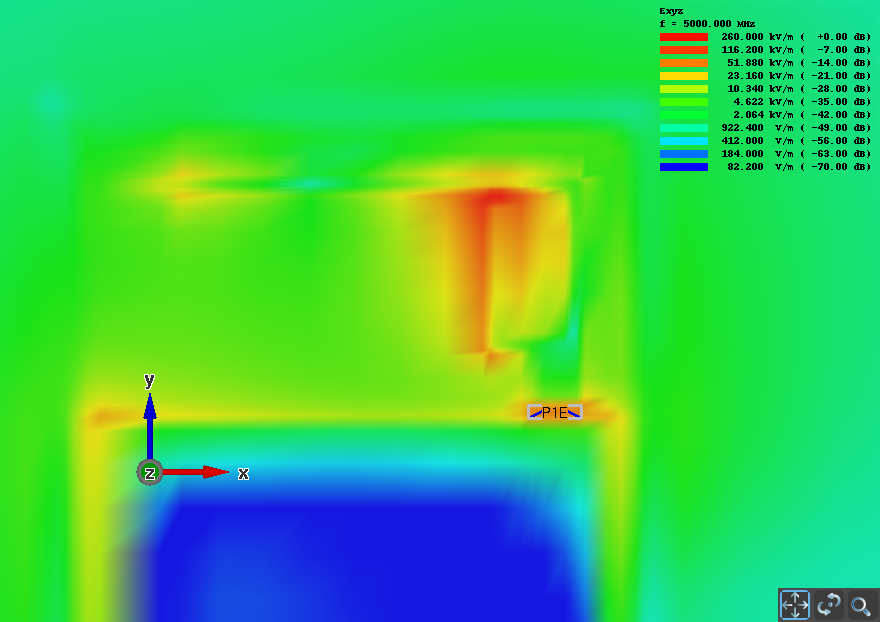
\includegraphics[width=1\textwidth]{../fig/plt/crazy_stuff_l4_pcb_v2c_laptop_1a_105_5ghz_3d_electric_field_xy.png}
				\caption{bei 5.0 GHz}
				\label{fig:electricfield_5_0}
			\end{center}
		\end{subfigure}
		\caption{Elektrisches Feld}
		\label{fig:electricfield}
	\end{center}
\end{figure}

\subsubsection{Oberflächenstromdichte}
\begin{figure}[h!]
	\begin{center}
		\begin{subfigure}[t]{0.49\textwidth}
			\begin{center}
				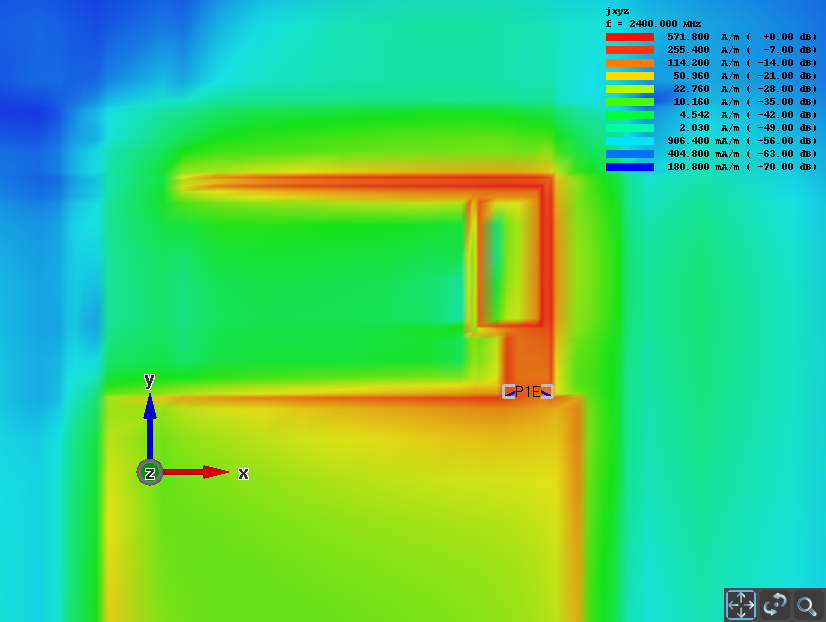
\includegraphics[width=0.94\textwidth]{../fig/plt/crazy_stuff_l4_pcb_v2c_laptop_1a_105_2ghz4_3d_surface_current_density_xy.png}
				\caption{bei 2.4 GHz}
				\label{fig:currentdensity_2_4}
			\end{center}
		\end{subfigure}
		\begin{subfigure}[t]{0.49\textwidth}
			\begin{center}
				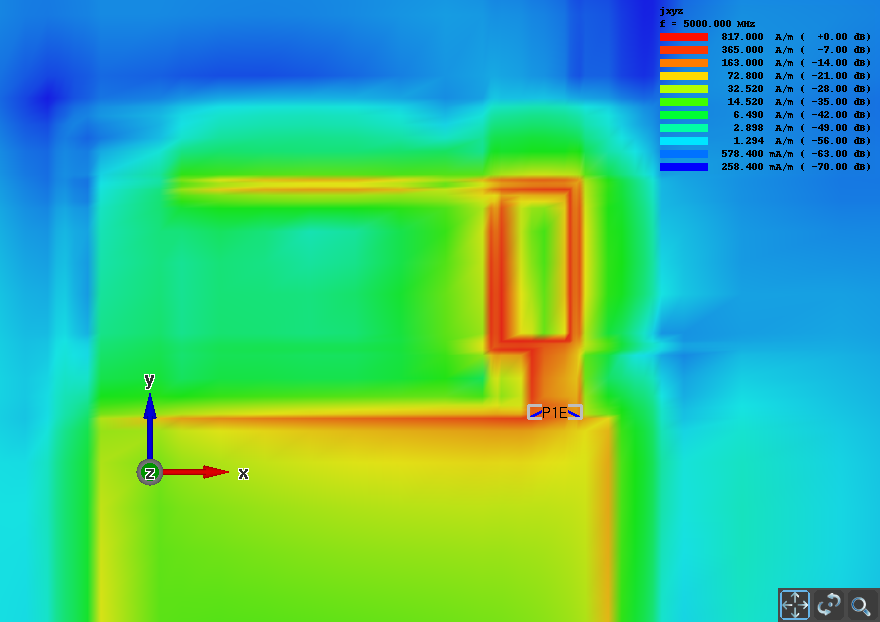
\includegraphics[width=1\textwidth]{../fig/plt/crazy_stuff_l4_pcb_v2c_laptop_1a_105_5ghz_3d_surface_current_density_xy.png}
				\caption{bei 5.0 GHz}
				\label{fig:currentdensity_5_0}
			\end{center}
		\end{subfigure}
		\caption{Oberflächenstromdichte}
		\label{fig:currentdensity}
	\end{center}
\end{figure}

\newpage
\subsubsection{Fernfeld bei 2.4 GHz}
In die Simulation wurde ein Laptopmodell miteinbezogen, in welchem der USB-Dongle eingesteckt war. Der Bildschirm wurde mit einem Öffnungswinkel von 105° simuliert.

\begin{figure}[h!]
	\centering
	\begin{subfigure}[b]{0.75\textwidth}
		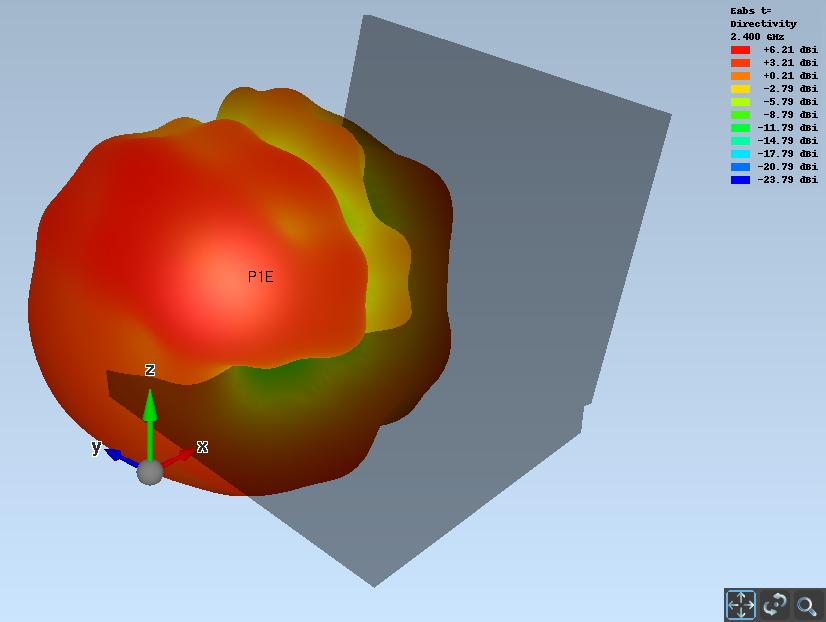
\includegraphics[width=1\textwidth]{../fig/plt/crazy_stuff_l4_pcb_v2c_laptop_1a_105_2ghz4_3d_farfield_eabs_xyz.png}
		\caption{$\vec{E}_{\mathrm{abs}}$}
	\end{subfigure}
	
	\vspace{3mm}
	
	\begin{subfigure}[b]{0.48\textwidth}
		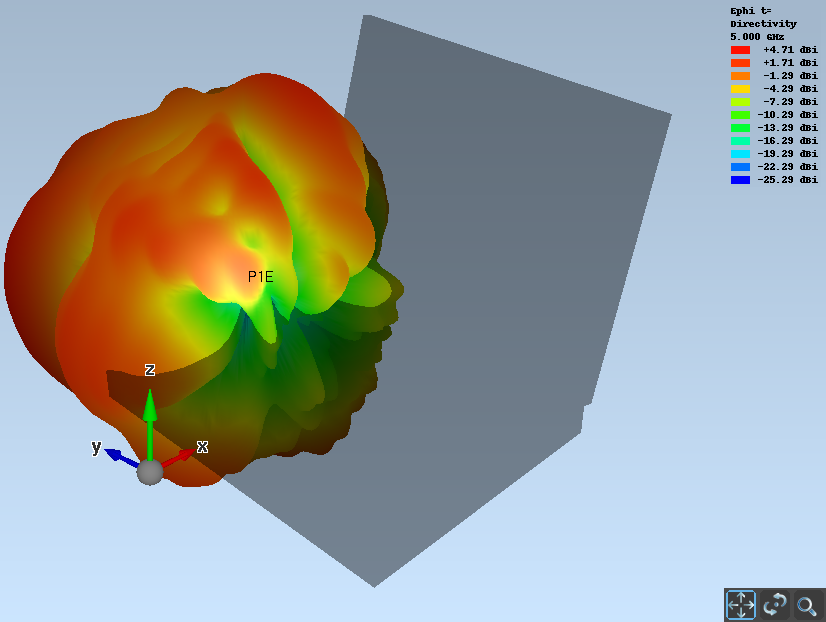
\includegraphics[width=1\textwidth]{../fig/plt/crazy_stuff_l4_pcb_v2c_laptop_1a_105_2ghz4_3d_farfield_ephi_xyz.png}
		\caption{$\vec{E}_{\varphi}$}
	\end{subfigure}
	\begin{subfigure}[b]{0.48\textwidth}
		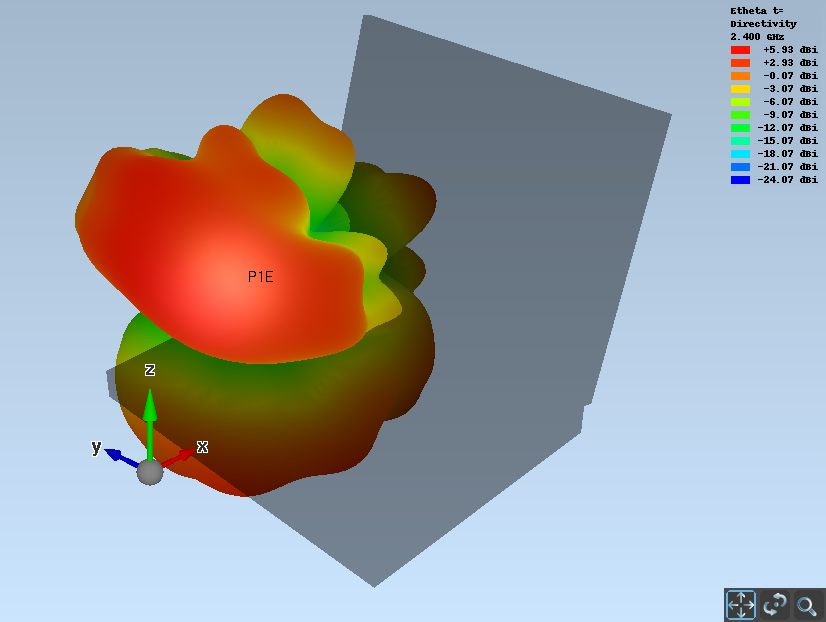
\includegraphics[width=1\textwidth]{../fig/plt/crazy_stuff_l4_pcb_v2c_laptop_1a_105_2ghz4_3d_farfield_etheta_xyz.png}
		\caption{$\vec{E}_{\Theta}$}
	\end{subfigure}
	\caption{$\vec{E}$ Fernfeldanalyse (3D) bei 2.4 GHz}
\end{figure}


\clearpage
\subsubsection{Fernfeld bei 5 GHz}
\begin{figure}[h!]
	\centering
	\begin{subfigure}[b]{0.75\textwidth}
		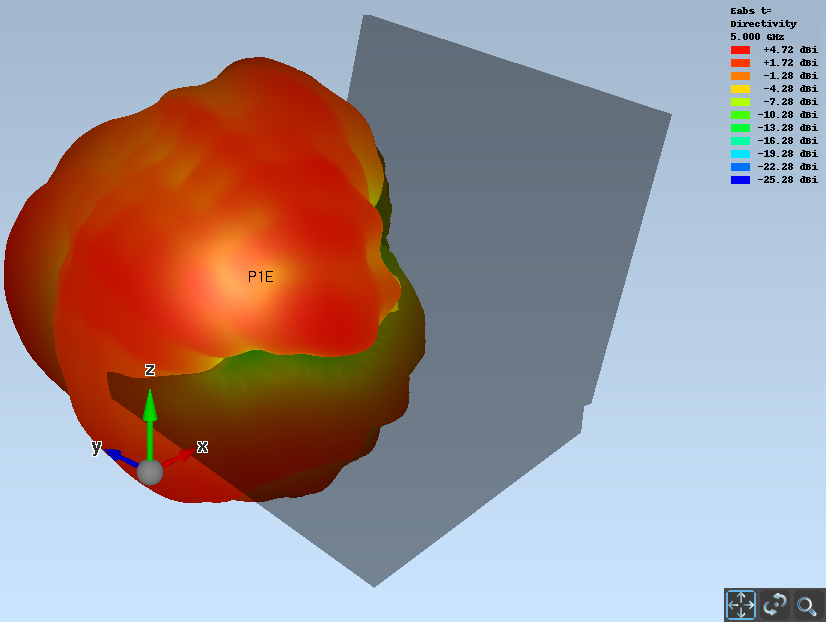
\includegraphics[width=1\textwidth]{../fig/plt/crazy_stuff_l4_pcb_v2c_laptop_1a_105_5ghz_3d_farfield_eabs_xyz.png}
		\caption{$\vec{E}_{\mathrm{abs}}$}
	\end{subfigure}

	\begin{subfigure}[b]{0.48\textwidth}
		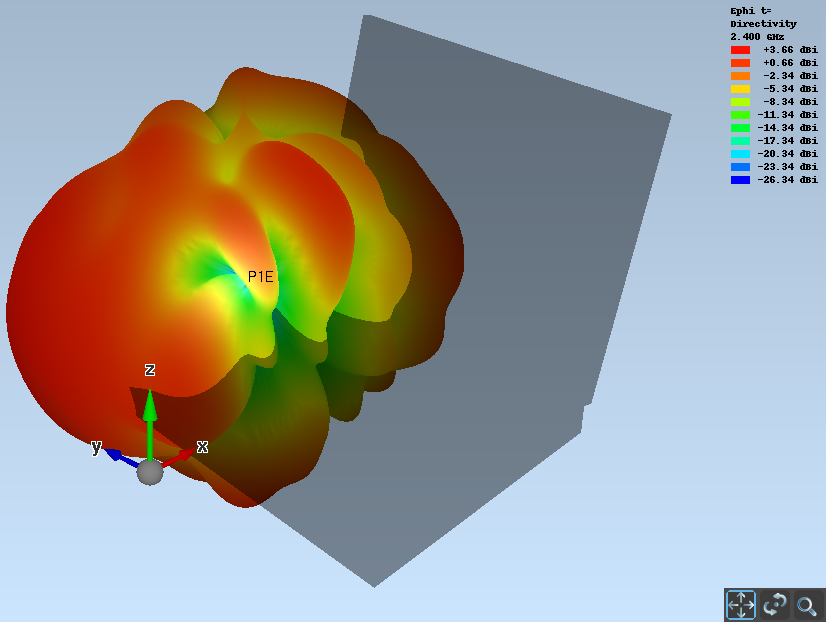
\includegraphics[width=1\textwidth]{../fig/plt/crazy_stuff_l4_pcb_v2c_laptop_1a_105_5ghz_3d_farfield_ephi_xyz.png}
		\caption{$\vec{E}_{\varphi}$}
	\end{subfigure}
	\begin{subfigure}[b]{0.48\textwidth}
		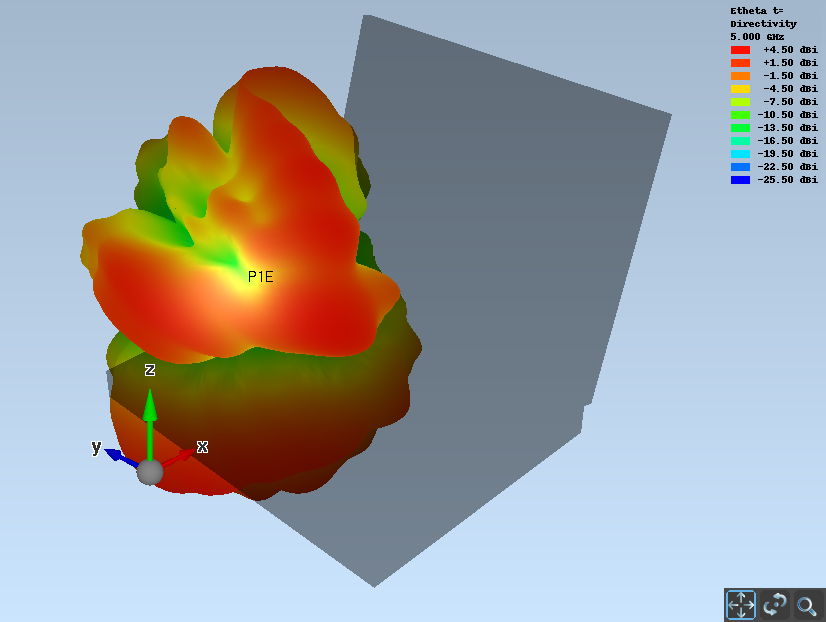
\includegraphics[width=1\textwidth]{../fig/plt/crazy_stuff_l4_pcb_v2c_laptop_1a_105_5ghz_3d_farfield_etheta_xyz.png}
		\caption{$\vec{E}_{\Theta}$}
	\end{subfigure}
	\caption{$\vec{E}$ Fernfeldanalyse (3D) bei 5.0 GHz}
\end{figure}


